\chapter{Object reconstruction}
\chaptermark{Object reconstruction}  
\thispagestyle{plain}  % First page has default style
\pagestyle{chapterpages}
\label{Section:Chapter4}
\minitoc

This chapter presents the reconstruction of physics objects in the CMS detector, which is foundational to all analyses performed in this thesis. In particular, $\PGt$ lepton reconstruction is a central focus. The reconstruction of $\PGt$ leptons is particularly challenging due to their short lifetime and complex decay modes, which can involve a mix of charged and neutral hadrons, electrons, muons, and undetectable neutrinos. Therefore, accurate $\PGt$ identification requires the excellent performance of multiple reconstruction components, including \textit{charged-particle tracking}, \textit{electromagnetic} and \textit{hadronic calorimetry}, \textit{muon identification}, and \textit{displaced secondary vertexing}.

However, operating in a high-multiplicity environment introduces additional challenges for the reconstruction and identification of physics objects. There is no guarantee that a reconstructed particle corresponds to a genuine physics object; such cases are referred to as \textit{misidentified} or \textit{``fake'' objects}. For example, jets initiated by quarks or gluons can sometimes be misidentified as hadronic $\PGt$ decays; leptons originating from heavy-flavour decays within jets may mimic prompt electrons or muons; and, conversely, muons and electrons can occasionally be misidentified as jets. To mitigate these effects, object identification algorithms incorporate \textit{multivariate discriminants} and \textit{\acp{WP}} that are tuned to balance efficiency and misidentification rates. However, in some cases, these strategies only partially suppress such backgrounds.

\section{Track reconstruction}

The first stage of the reconstruction process, known as \textbf{local reconstruction}~\cite{CMS_TrackerPerformance_2014,CMS_Track_Reconstruction_Run2_3}, involves clustering zero-suppressed signals above predefined thresholds in the tracker sensors to form hits, referred to as \textit{clusters}. For each cluster, both the position and its associated uncertainty are estimated within a local coordinate system defined by the sensor geometry. These locally reconstructed hits form the basis for the subsequent \textbf{global reconstruction}~\cite{CMS_TrackerPerformance_2014,CMS_Track_Reconstruction_Run2_3} of particle trajectories.

Global track reconstruction at CMS is facilitated by the \textbf{\ac{CTF}} algorithm~\cite{CMS_TrackerPerformance_2014,CMS_Track_Reconstruction_Run2_3}, an adaptation of the combinatorial \textit{\ac{KF}}~\cite{KF_1,KF_2,KF_3}\footnote{KF~\cite{KF_4} is recursive algorithm that uses a series of measurements over time to estimate the state of a system. This is done by estimating a joint probability distribution over the variables of interest at each time step.} approach. This adaptation enables pattern recognition and track fitting to be performed within a unified framework, allowing hits to be incrementally added and track parameters to be continuously updated in a process known as \textbf{iterative tracking}. A single iteration of the CTF algorithm proceeds in four steps:

\begin{enumerate}
    \item \textbf{Seed generation}: Initial track candidates are formed using a small number of hits (typically two or three) in the innermost layers of the tracker. Each \textit{seed} provides an initial estimate of the particle's trajectory parameters, such as position, direction, and momentum, as well as their associated uncertainties. 
    \item \textbf{Track finding}: Seed trajectories are extrapolated along the expected trajectory of a charged particle using a Kalman Filter (KF). At each detector layer, additional hits along the expected flight path are identified and associated with the track candidate; the trajectory parameters are then updated accordingly. This process is repeated iteratively until the outermost layer of the detector is reached, gradually building complete track candidates from the initial seeds.
    \item \textbf{Track fitting}: The final trajectory is refitted iteratively to improve the estimate of the track parameters. This is done using a combination of a KF and a smoother, incorporating all available hit information.
    \item \textbf{Track selection}: Tracks are required to pass a set of quality flags.
\end{enumerate}

The \textbf{iterative tracking} procedure in CMS is performed in six successive iterations, each designed to target different classes of tracks. The initial iterations target tracks that are the easiest to find (\eg high $p_\mathrm{T}$ tracks, and tracks produced near the primary interaction point). After each iteration, the combinatorial complexity is reduced by removing hits associated with tracks. This enables later iterations to target more challenging classes of tracks (\eg low $p_\mathrm{T}$ tracks, and tracks displaced from the interaction point). 

\section{Vertex reconstruction}

The primary goal of the CMS vertex reconstruction~\cite{CMS_TrackerPerformance_2014} is to determine the positions and associated uncertainties of all proton-proton interaction vertices in an event, including both the \textit{\ac{PV}} (associated with the \textit{``signal'' interaction}) and any additional vertices originating from \textit{PU} collisions, using all available reconstructed tracks. The reconstruction process is performed in three main steps: 

\begin{itemize}
    \item \textbf{Track selection}: Tracks consistent with originating promptly near the centre of the luminous region (referred to as the beam spot) are selected. This selection is based on applying quality requirements to the tracks, such as cuts on the transverse impact parameter significance relative to the beam spot and minimum numbers of associated pixel and strip hits.
    \item \textbf{Track clustering}: Tracks are clustered into groups that appear to be originating from the same vertex. This clustering is performed based on their z-coordinate at the point of closest approach to the beam spot using a \textit{deterministic annealing algorithm}~\cite{DeterministicAnnealing}.
    \item \textbf{Vertex fitting}: Candidate vertices composed of at least two tracks are fitted using an \textit{adaptive vertex fitter}~\cite{VertexFitting_2006,VertexFitting_2007} to determine the best estimate of the vertex parameters. These parameters include the $x$, $y$, and $z$ positions, the associated covariance matrix, and indicators of fit quality. Additionally, the adaptive fit assigns a weight between 0 and 1 to each track, reflecting the probability that the track is genuinely associated with the vertex.
\end{itemize}

Once all the vertices are reconstructed, a collection is formed, which is ordered by the quadratic sum of the transverse track momenta associated with each vertex, $\sum_{\text{tracks}} p_{\mathrm{T}}^2$. The vertex with the largest sum is assumed to most likely correspond to the vertex of the hard scattering process~\cite{ParticleFlow}. The efficiency to correctly identify the PV when at least three tracks are associated is close to 100\%~\cite{CMS_TrackerPerformance_2014}. The resolution of the PV position, particularly in the $x$ and $z$ coordinates, has been measured using $\sqrt{s} = 13\ \mathrm{TeV}$ collision data~\cite{PrimaryVertex_Resolution} and is found to improve rapidly as the summed $p_{\mathrm{T}}$ of the associated tracks increases, as shown in Fig.~\ref{Figure:Chapter4_PrimaryVertex_Resolution}.

\begin{figure}[h]
    \centering
    % First row
    \begin{subfigure}[b]{0.49\textwidth}
        \centering
        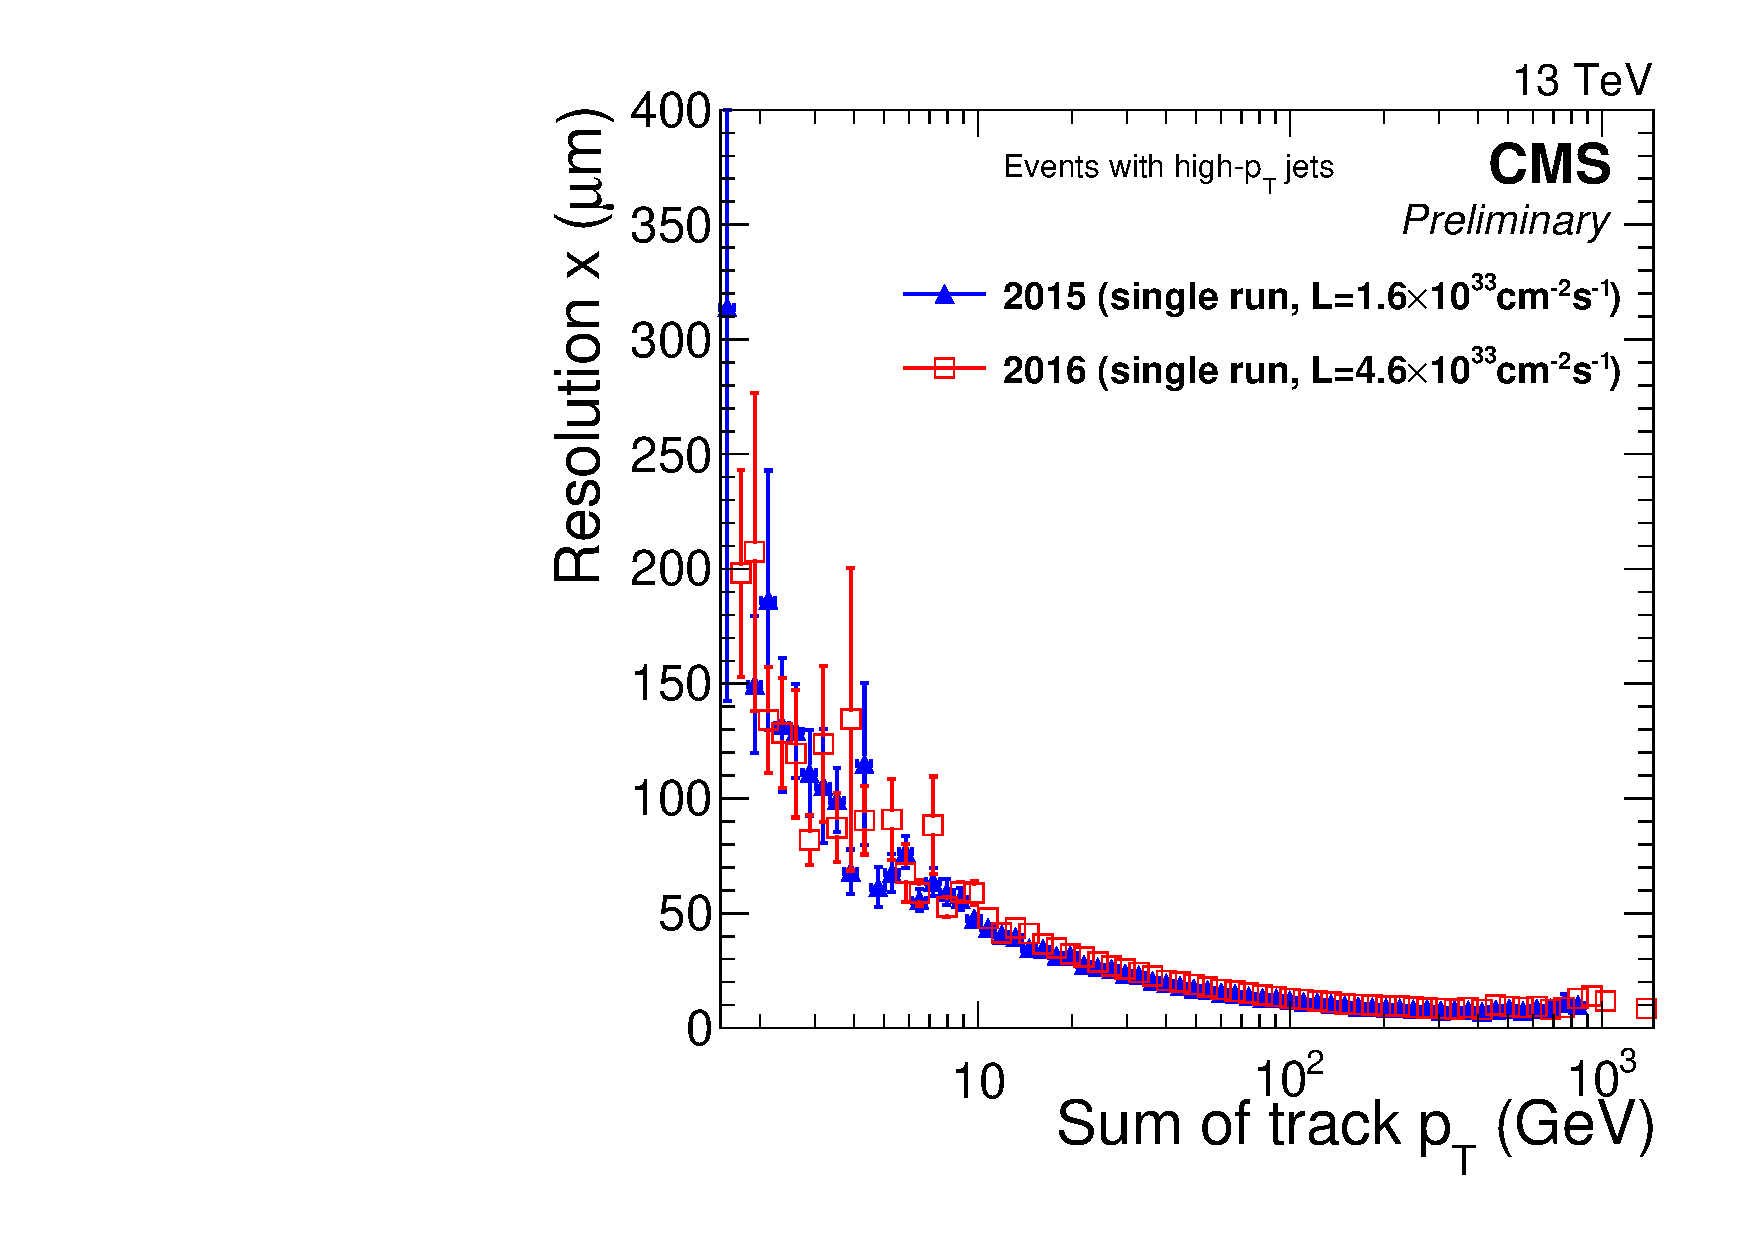
\includegraphics[width=\textwidth]{Figures/Chapter4/resolution_sumpt_x.pdf}
        \caption{}
    \end{subfigure}
    \begin{subfigure}[b]{0.49\textwidth}
        \centering
        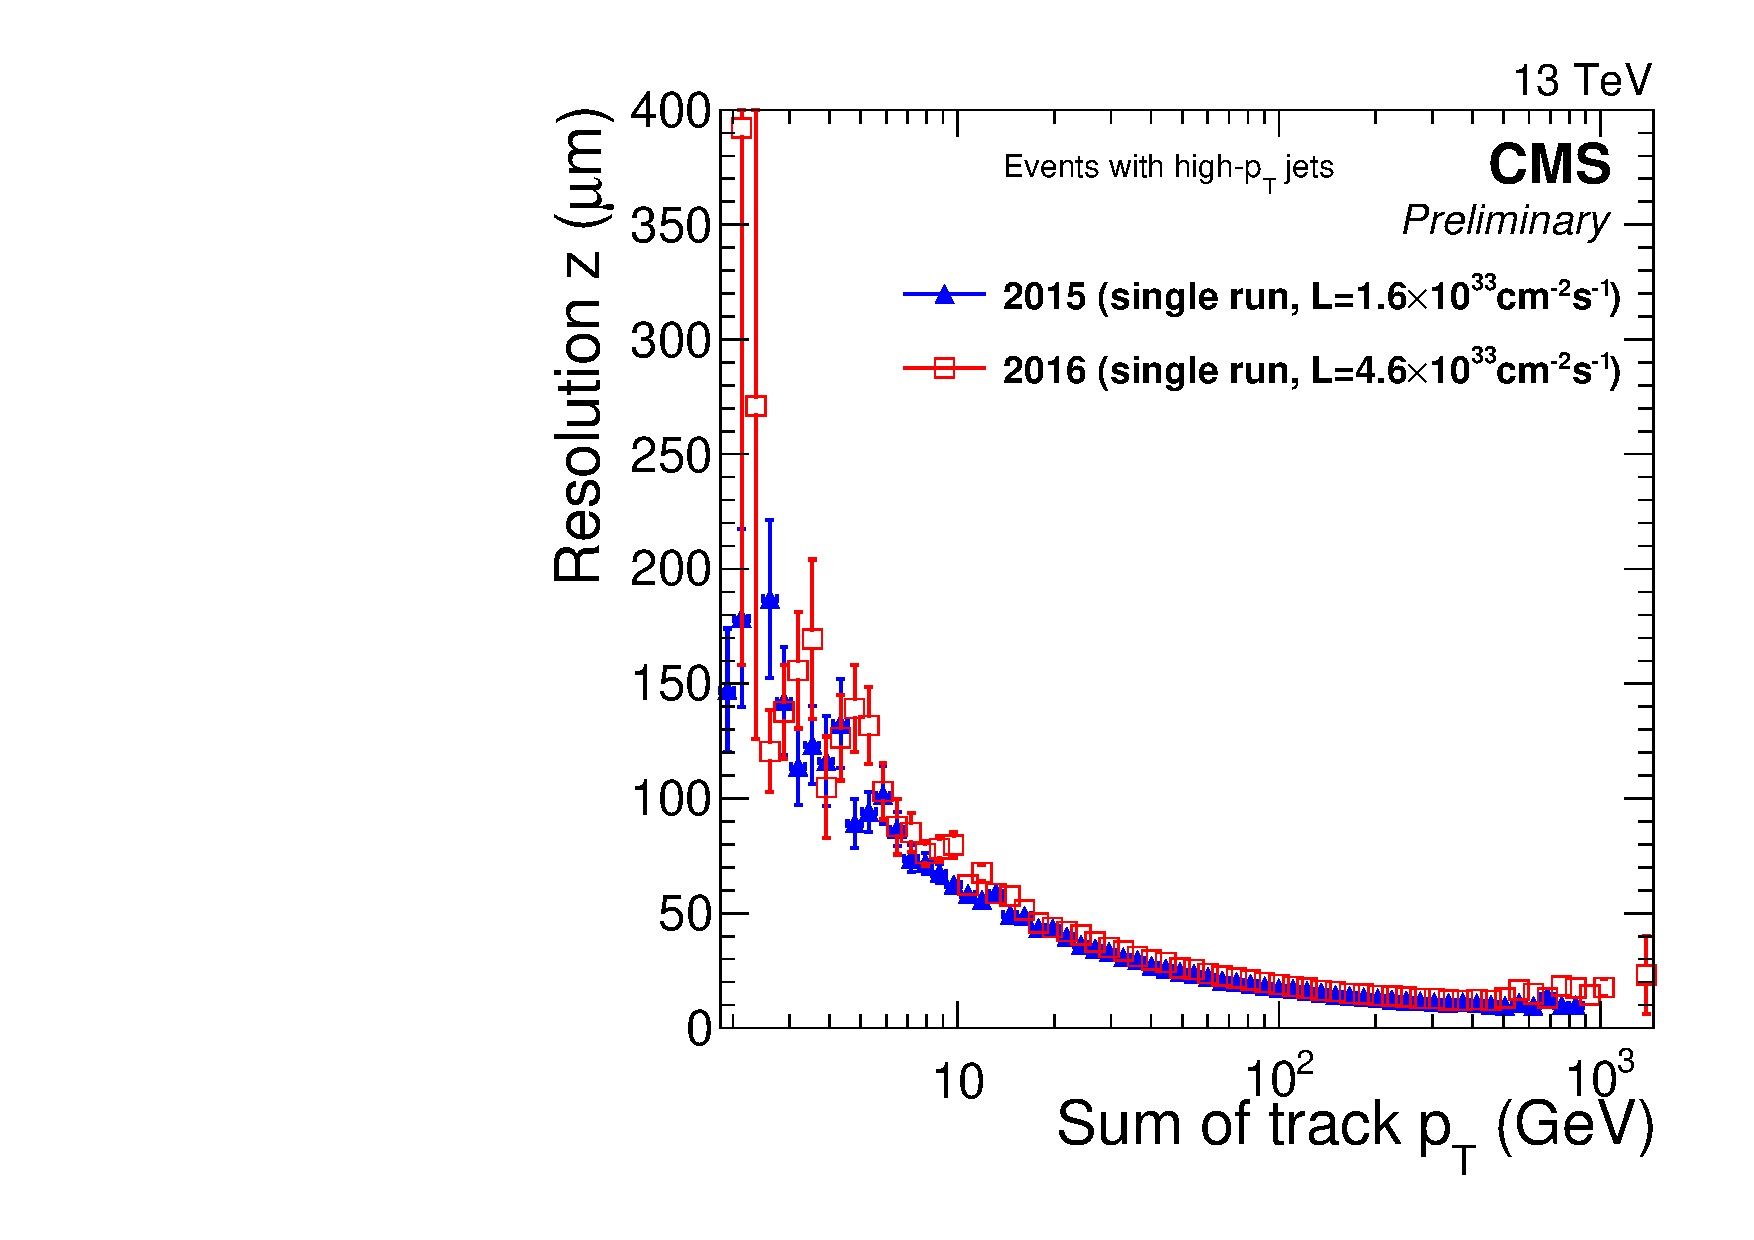
\includegraphics[width=\textwidth]{Figures/Chapter4/resolution_sumpt_z.pdf}
        \caption{}
    \end{subfigure}
\caption[Resolution of the reconstructed transverse and longitudinal positions of the primary vertex using CMS collision data (2015 \& 2016)]{Resolution of the reconstructed PV position in the \textbf{(a)} transverse ($x$) and \textbf{(b)} longitudinal ($z$) directions as a function of the $\sum p_\mathrm{T}$ of the associated tracks. Measurements are shown for pp collisions recorded in 2015 (blue) and 2016 (red). Figures taken from Ref.~\cite{PrimaryVertex_Resolution}.}

\label{Figure:Chapter4_PrimaryVertex_Resolution}
\end{figure}

\section{Particle flow}

\section{Muons}

\section{Electrons}

\section{Jets}

\section{Missing transverse energy}

\section{Taus}